\documentclass[article, oneside]{ufpethesis}

\usepackage{pdfpages}
\usepackage{listings}
\usepackage{xcolor}
\usepackage{paralist}
\usepackage[style=ieee]{biblatex}
\usepackage{csquotes}
\definecolor{codegreen}{rgb}{0,0.6,0}
\definecolor{codegray}{rgb}{0.5,0.5,0.5}
\definecolor{codepurple}{rgb}{0.58,0,0.82}
\definecolor{backcolour}{rgb}{0.95,0.95,0.92}
\lstdefinestyle{mystyle}{
    backgroundcolor=\color{backcolour},
    commentstyle=\color{codegreen},
    keywordstyle=\color{magenta},
    numberstyle=\tiny\color{codegray},
    stringstyle=\color{codepurple},
    basicstyle=\ttfamily\footnotesize,
    breakatwhitespace=false,
    breaklines=true,
    captionpos=b,
    keepspaces=true,
    numbers=left,
    numbersep=5pt,
    showspaces=false,
    showstringspaces=false,
    showtabs=false,
    tabsize=2
}
\lstset{style=mystyle}

\addbibresource{library.bib}

\institute{Centro de Informática}
\program{Bacharelado em Ciência da Computação}
\majorfield{Ciência da Computação}
\author{José Gabriel Silva Pereira}
\adviser{Paulo Henrique Monteiro Borba}
\coadviser[f]{Paola Rodrigues de Godoy Accioly}
\title{Análise de extensão do CSDiff para uso em linguagens com poucos separadores sintáticos}
\date{27 de Abril de 2023}

\begin{document}
\frontmatter
\frontpage
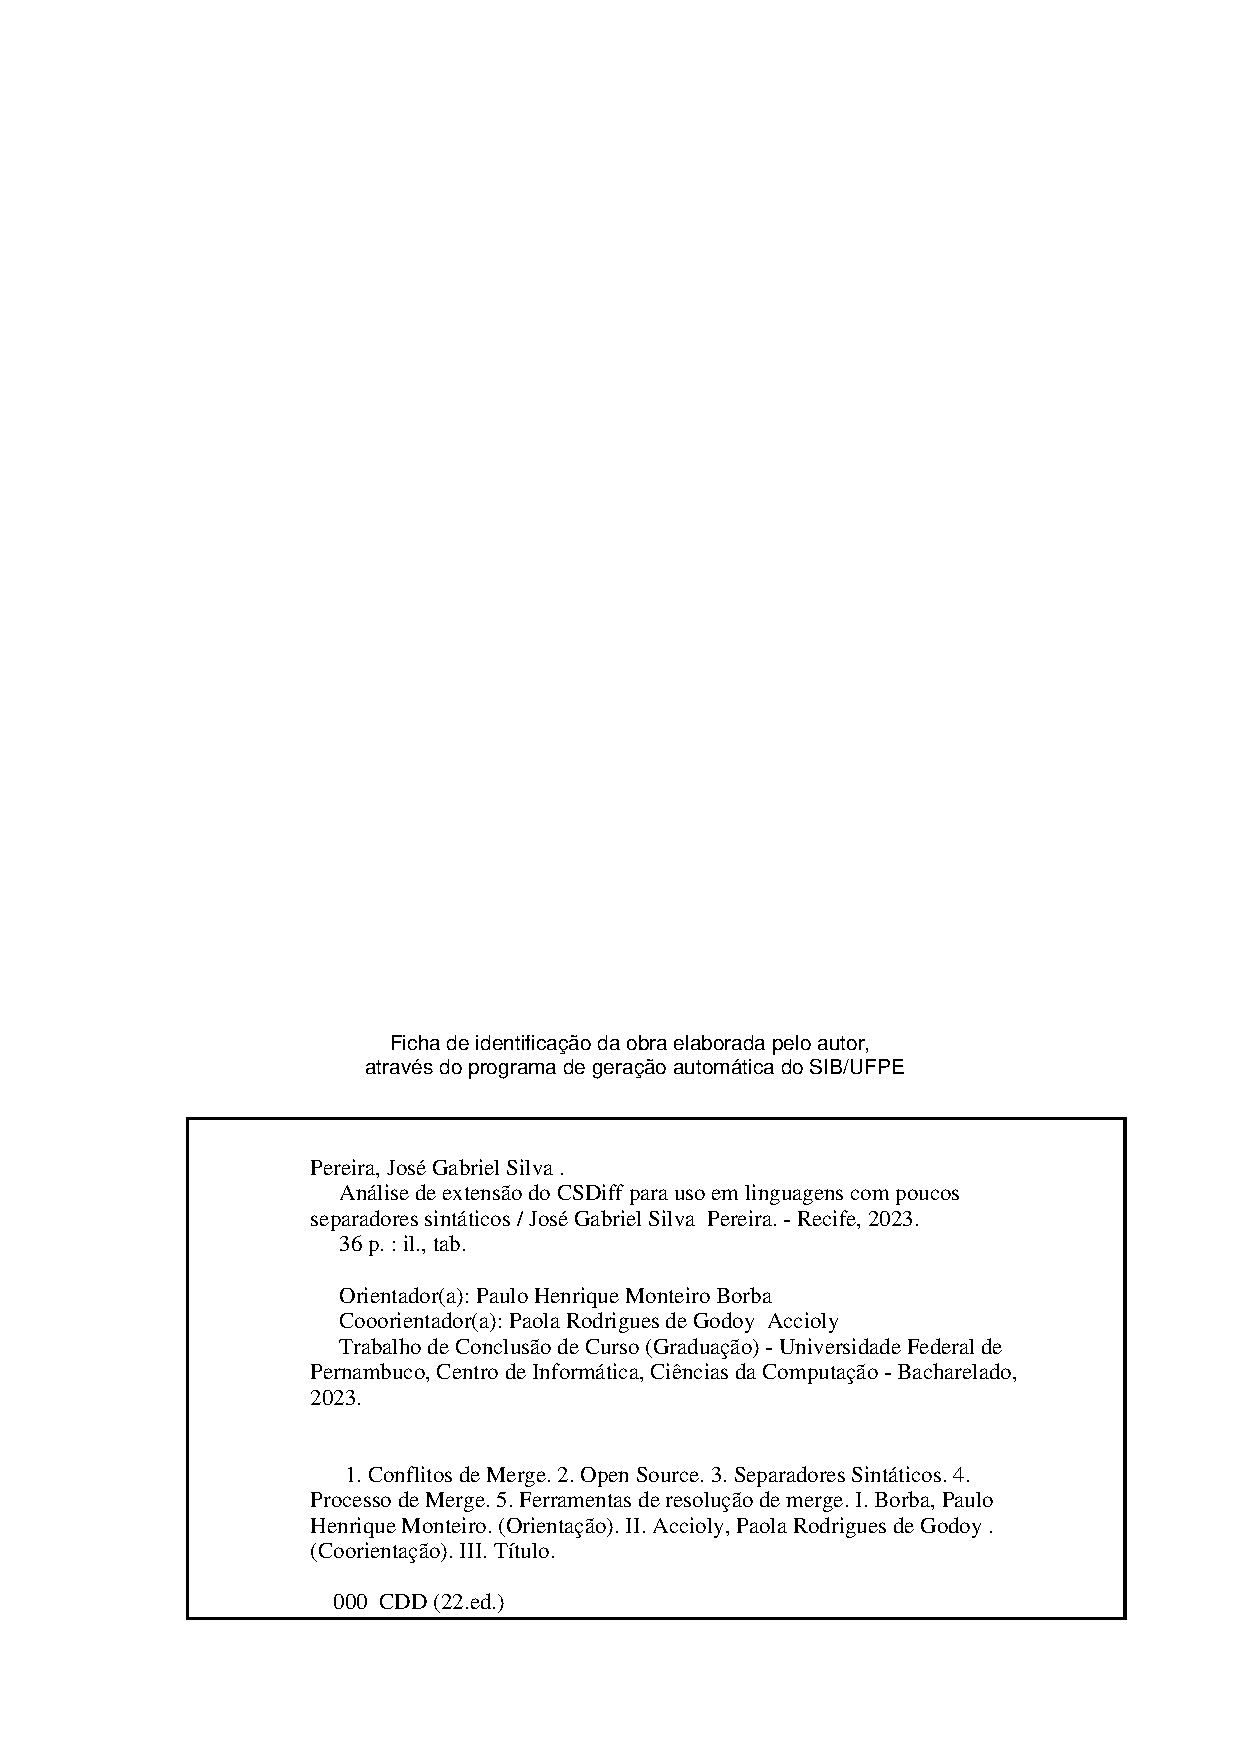
\includepdf[]{ficha.pdf}
\presentationpage

% \acknowledgements
TODO: agradecimentos

\resumo
A prática de desenvolvimento de software, há muito tempo deixou de ser uma tarefa
que era realizada por somente uma pessoa, pois, com o avanço da tecnologia, sistemas
cada vez mais complexos foram sendo criados fazendo com que muitas pessoas trabalhassem no
mesmo projeto. Por conta disso, ferramentas de controle de versionamento de
código foram criadas, permitindo que múltiplos desenvolvedores trabalhassem modificando
o mesmo trecho de código simultaneamente. Porém, essas modificações simultâneas
podem gerar conflitos quando feitas em um mesmo pedaço de código, o que impacta
negativamente na produtividade de um time. Ao decorrer do tempo, diversas formas
de como detectar conflitos na junção de versão de códigos foram criadas, dentre
elas: linha a linha, estruturada e semiestruturada. Neste trabalho,
é proposto uma extensão para uma ferramenta semiestruturada de detecção de conflitos
ja existente, o \emph{CSDiff} \cite{clementino2021textual}, de forma que ela
utilize indentação como separador da linguagem, permitindo assim que, durante a
detecção de conflitos em linguagens com poucos separadores sintáticos, ainda seja
possivel permitir uma redução de falsos conflitos, consequentemente melhorando a
produtividade de um time.
\begin{keywords}
	Processo de Merge, Desenvolvimento Colaborativo, Merge Textual, Merge
	Estruturado, Separadores sintáticos
\end{keywords}

\abstract
The practice of software development has long ceased to be a task performed by
only one person, as with the advancement of technology, increasingly complex
systems have been created, causing many people to work on the same project.
Therefore, code version control tools were created, allowing multiple developers
to work on modifying the same piece of code simultaneously. However, these simultaneous
modifications can generate conflicts when made on the same piece of code, negatively
impacting a team's productivity. Over time, several ways of detecting conflicts
in the merging of code versions have been created, including line-by-line, structured,
and semi-structured. In this work, an extension is proposed for an existing
semi-structured conflict detection tool, the \emph{CSDiff} \cite{clementino2021textual},
so that it uses indentation as a language separator, thus allowing, during
conflict detection in languages with few syntactic separators, a reduction in
false conflicts, consequently improving a team's productivity.
\begin{keywords}
	Merge Process, Collaborative Development, Textual Merge, Structured Merge, Syntactic Separators.
\end{keywords}



% \tableofcontents
% \listoffigures
% \listoftables

\mainmatter
% \verb#\part# $\supset$ \verb#\section# $\supset$
% \verb#\section# $\supset$ \verb#\subsection# $\supset$
% \verb#\subsubsection# $\supset$ \verb#\paragraph#.
\chapter{Introdução}

Com o crescimento da complexidade dos sistemas de software, surge a necessidade
de que múltiplas pessoas trabalhem num mesmo projeto. Essas modificações, com o
objetivo de trazer mais produtividade, costumam ser executadas de forma
paralela e podem acontecer em trechos de código em comum. Tendo como objetivo
auxiliar os desenvolvedores a controlar e versionar suas modificações no
código, ferramentas de controle de versão de código foram criadas. Essas
ferramentas auxiliam a reduzir o trabalho extra quando se trata de modificações
paralelas que precisam ser unidas. O processo de unir duas modificações
paralelas de código é chamado de \emph{merge}~\cite{mens02}.

No processo de \emph{merge}, quando dois desenvolvedores modificam o mesmo
trecho de código e essas mudanças interferem uma na outra, é gerado um
conflito. Esses conflitos, quando detectados, algumas vezes precisam ser
resolvidos por um ou ambos os desenvolvedores, o que acaba impactando na
produtividade, dado que resolvê-los geralmente é uma tarefa que geralmente
demanda tempo~\cite{brun11}. Além do impacto na produtividade do time, quando
esses conflitos não são detectados pela ferramenta de \emph{merge}, ou quando
são detectados e mal resolvidos, eles podem levar à introdução de bugs dentro
do código, o que influencia na qualidade do produto final~\cite{brin20}.

A abordagem de \emph{merge} mais utilizada na indústria atualmente é o
\emph{merge} não estruturado~\cite{khan07}, que se utiliza de uma análise
puramente textual, equiparando linha a linha trechos do código para detectar e
resolver conflitos. Porém, por não utilizar a estrutura do código que está
sendo integrado, muitas vezes essa abordagem gera falsos conflitos. Ao
observar isso, pesquisadores propuseram ferramentas que se baseiam na estrutura
dos arquivos que estão sendo integrados, criando uma árvore sintática a partir
do texto dos arquivos e de sua linguagem de programação~\cite{apel11}. Essas
abordagens são chamadas estruturadas e semiestruturadas.

Em estudos anteriores~\cite{apel11,cavalcanti15,cavalcanti19}, as duas
abordagens (estruturada e semiestruturada) foram comparadas em relação à não
estruturada e mostrou-se que, para a maioria das situações de \emph{merge} dos
projetos, houve uma redução de conflitos em favor da semi ou da estruturada.
Essa redução se dá por conta de falsos conflitos que possuem resolução óbvia,
como por exemplo, quando os desenvolvedores adicionam dois métodos diferentes e
independentes numa mesma região do código~\cite{cavalcanti17}.

Esse benefício advém da exploração da estrutura gerada pela análise sintática,
também chamada de análise gramatical. Ela envolve o agrupamento dos tokens
(palavras) do programa fonte em frases. Cada linguagem possui conjuntos de
tokens, onde alguns servem como divisores de elementos sintáticos e escopo
semântico, como por exemplo as chaves ('\verb|{|', '\verb|}|') numa linguagem como Java.
Estes tokens são definidos aqui como
\textbf{separadores} sintáticos.

A solução não estruturada mais utilizada, o \emph{Diff3}, se baseia somente na
quebra de linha como o divisor de contexto para detecção de conflitos. Assim, o
algoritmo de \emph{merge} compara as linhas mantidas, adicionadas, e removidas
por cada desenvolvedor e, com base nisso, reporta conflito quando as mudanças
ocorrem em uma mesma área do texto, isto é, uma área onde não há uma mesma
linha (ou linhas consecutivas) mantida que separa as mudanças feitas pelos dois
desenvolvedores.

Como forma de melhorar os resultados do \emph{Diff3}, o \emph{CSDiff}, proposto
em trabalhos anteriores~\cite{clem21}, utiliza-se dos separadores mencionados
acima para dividir o contexto de cada linha de código. Assim, o algoritmo de
\emph{merge} consegue, por exemplo, resolver conflitos em uma mesma linha,
contanto que esses conflitos estejam separados por pelo menos um dos
separadores definidos.

Apesar de funcionar bem para linguagens como Java, o \emph{CSDiff} possui
limitações, pois linguagens como Python, possuem poucos separadores (seu
principal separador é a própria indentação do código, que não é considerado
pelo \emph{CSDiff} atual). Este trabalho propõe uma modificação para o
\emph{CSDiff}, que utiliza a indentação como um separador sintático, de forma a
tentar resolver esse problema, e analisa os resultados em comparação ao
\emph{merge} não estruturado puramente textual. Em particular, investiga-se as
seguintes perguntas de pesquisa:

\begin{compactenum}[1)]
	\item PP1: A nova solução de \emph{merge} não estruturado, utilizando indentação,
	reduz a quantidade de conflitos reportados em comparação ao \emph{merge} puramente textual?
	\item PP2: A nova solução de \emph{merge} não estruturado, utilizando indentação,
	reduz a quantidade de cenários com conflitos reportados em comparação ao \emph{merge} puramente textual?
	\item PP3: A nova solução de \emph{merge} não estruturado, utilizando indentação,
	reduz a quantidade de falsos conflitos e cenários com falsos conflitos reportados
	(falsos positivos) em comparação ao \emph{merge} puramente textual?
	\item PP4: A nova solução de \emph{merge} não estruturado, utilizando indentação,
	amplia a possibilidade de comprometer a corretude do código, por aumentar o número de
	integrações de mudanças que interferem uma na outra, sem reportar conflitos (falsos negativos),
	além de aumentar cenários com falsos negativos?
	\item PP5: A nova solução de \emph{merge} não estruturado, utilizando indentação,
	demonstra um aumento de produtividade considerando o ato de resolver conflitos de merge?
\end{compactenum}

Os resultados obtidos mostram que além de aumentar a quantidade de conflitos
reportados (como esperado considerando os resultados dos trabalhos anteriores),
o \emph{merge} não estruturado utilzando separadores e indentação, demonstra,
para a amostra utilizada, um aumento de cenários \emph{aFN} (Falsos Negativos
Adicionados, ou seja, cenários onde a ferramenta resolveu conflitos de forma
errada, enquanto a ferramenta \emph{Diff3} resolveu corretamente) proporcional
a quantidade de cenários \emph{aFP} (Falsos Positivos Adicionados, ou seja,
cenários onde a ferramenta reportou conflitos enquanto a ferramenta Diff3 não
reportou nenhum e seu resultado era igual ao do merge do repositório) reduzido
quando comparado ao \emph{Diff3}.

Por outro lado, ao se fazer a análise de aumento de produtividade considerando
o ato de resolver e reduzir conflitos, além de considerar geração de falsos
conflitos reais e resolução errada de conflitos, notou-se um bom aumento de
produtividade com a utilização do \emph{CSDiff} original, enquanto que o
\emph{CSDiff} modificado demonstrou um resultado levemente pior. Os conceitos
utilizados para esta análise são explicados na seção~\ref{concept_PP5}.



\chapter{Motivação}
\section{Merge Não Estruturado}
Apesar da evolução dos sistemas de controle de versão, as ferramentas
utilizadas para realizar \emph{merge} não evoluiram tanto. A ferramenta mais
utilizada atualmente é o \emph{Diff3}~\cite{mens02}, que consiste em uma
abordagem puramente textual baseada em linhas. Essa ferramenta, ao receber os
três arquivos que configuram o cenário de merge (chamemos de \emph{base},
\emph{left} e \emph{right}), compara, linha a linha, as duas versões
modificadas (\emph{left} e \emph{right}) com seu ancestral comum (\emph{base}),
que foi o arquivo que deu origem às modificações que vão ser integradas. Após
isso, a ferramenta agrupa as maiores áreas em comum e checa se existem
interseções entre as áreas modificadas por \emph{left} e \emph{right}. Essas
interseções são definidas como conflitos de merge~\cite{khan07}, elas serão
sinalizadas pelo \emph{Diff3} através de marcadores
\verb|(``>>>>>>>``,``=======`` e ``<<<<<<<``)|, como demonstrado na
Figura~\ref{diff3_example}.

Por considerar as mudanças linha a linha para detectar os conflitos, muitas
vezes essa ferramenta relata falsos conflitos de modificações que alteram a
mesma linha ou linhas consecutivas, mas que não interferem entre si
semanticamente. Esse problema poderia ser resolvido utilizando ferramentas que
explorem a estrutura sintática do código em questão~\cite{cavalcanti19}

Para ilustrar esse problema causado pelo \emph{merge} não estruturado,
utilizamos a implementação de um método \detokenize{to_string} que recebe uma
lista de strings e retorna uma string juntando todos os elementos da lista
separados por dois \emph{underlines} \detokenize{(``__``)}. Observe que as
mudanças feitas pelo \emph{left} foram a adição de uma nova condição no
\emph{if}, e a mudança da string separadora do \emph{return} final (modificado
de ``..`` para \detokenize{``__``}). Por outro lado, as mudanças feitas pelo
\emph{right} foram o valor padrão de retorno de uma string vazia para uma
constante (por simplicidade consideramos que a constante foi definida na classe
onde o método está sendo implementado), e a mesma modificação que o \emph{left}
fez no último return do método. Perceba que todas essas mudanças são
independentes entre si, mas por elas acontecerem em linhas consecutivas, o
\emph{Diff3} relata todas elas em um mesmo conflito
(Figura~\ref{diff3_example}).

\begin{figure}[ht]
	\begin{center}
		\lstinputlisting[language=Python]{./example/no_indentation/base.py}
		\caption{Arquivo \emph{base} que contém o método \detokenize{to_string}}\label{base_example}
	\end{center}
\end{figure}

\begin{figure}[ht]
	\begin{center}
		\lstinputlisting[language=Python]{./example/no_indentation/left.py}
		\caption{Arquivo \emph{left} que contém o método \detokenize{to_string}}\label{left_example}
	\end{center}
\end{figure}

\begin{figure}[ht]
	\begin{center}
		\lstinputlisting[language=Python]{./example/no_indentation/right.py}
		\caption{Arquivo \emph{right} que contém o método \detokenize{to_string}}\label{right_example}
	\end{center}
\end{figure}

\begin{figure}[ht]
	\begin{center}
		\lstinputlisting[language=Python]{./example/no_indentation/diff3.py}
	\end{center}
	\caption{Resultado de executar o \emph{Diff3}}\label{diff3_example}
\end{figure}

\section{Merge Semiestruturado e Estruturado}
Como alternativa ao uso de merge não estruturado, existem as abordagens
semiestruturadas ou completamente estruturadas~\cite{cavalcanti19}. Ao
contrário da abordagem não estruturada, essas abordagens levam em consideração
a estrutura sintática da linguagem de programação para identificar conflitos
com maior precisão e resolvê-los de forma mais correta. Essas abordagens criam
árvores sintáticas para cada versão dos arquivos a serem integrados
(\emph{base}, \emph{left} e \emph{right}) e comparam essas árvores para
identificar nós comuns e adições ou remoções em cada árvore. Dessa forma, cada
elemento sintático é representado em nós distintos, e conflitos são sinalizados
quando as mudanças a serem integradas estão relacionadas ao mesmo nó da árvore.
Isso significa que, em vez de usar linhas como a unidade básica para
comparação, essas ferramentas usam nós sintáticos como unidade.

Essas ferramentas estruturadas e semiestruturadas conseguem evitar falsos
conflitos encontrados na abordagem não estruturada. Por exemplo, duas situações
em que dois desenvolvedores adicionam separadamente dois novos métodos com
diferentes assinaturas em uma mesma área do texto podem ser conciliadas com
sucesso. As mudanças ocorrem na mesma linha, mas cada declaração é representada
por um nó diferente, pois o identificador do método é parte do nó, e os dois
nós são mantidos na árvore resultante da integração.

Apesar da melhora em relação ao relato de falsos positivos,
Cavalcanti~\cite{cavalcanti17} argumenta que ferramentas semiestruturadas tendem
a gerar falsos negativos que são mais difíceis de detectar e resolver, além de
não encontrar evidências de que essas ferramentas reduzem a quantidade de
falsos negativos relatados em comparação a ferramentas não estruturadas.

Dessa forma, é fácil observar que uma ferramenta estruturada para Python
evitaria o conflito apresentado na Figura~\ref{diff3_example}. A ferramenta,
utilizando a estrutura da linguagem, identificaria que, apesar das mudanças
representadas na Figura~\ref{left_example} e na Figura~\ref{right_example}
ocorrerem em linhas consecutivas (o que faz com que o \emph{Diff3} agrupe as
mudanças em um único bloco de conflito), elas estariam associadas a nós
diferentes na árvore sintática. A ferramenta então juntaria as mudanças em uma
versão resultante que contém a nova condição proposta por \emph{left} e o novo
valor de retorno proposto por \emph{right}, evitando o falso conflito.

\section{Merge não Estruturado com separadores}

As abordagens estruturadas e semiestruturadas discutidas na seção anterior,
apesar benéficas em algumas situações, possuem um custo adicional, dado que elas se
baseiam em manipulação de árvores sintáticas, que por sua vez são dependentes
da linguagem em questão e demandam um esforço significativo de implementação
por linguagem, além de que a manipulação das árvores sintáticas possui um custo
computacional maior em relação a abordagens puramente textuais.

Para reduzir essas desvantagens, Clementino~\cite{clem21} propôe uma nova
ferramenta chamada \textbf{Custom Separators
	Diff}\footnote{https://github.com/JonatasDeOliveira/custom-separators-merge-tool/blob/main/csdiff.sh}
(\emph{CSDiff}), cujo funcionamento baseia-se na abordagem puramente textual,
mas que também considera a estrutura sintática do programa por meio de um
conjunto de separadores da linguagem, escolhidos pelo usuário e passados como
parâmetro.

\begin{center}
	\centering
	\begin{compactenum}[(1)]
		\item Transforma os arquivos \emph{base}, \emph{left} e
		\emph{right}, fazendo com que os separadores sintáticos dados
		como entrada fiquem em linhas separadas, adicionando uma linha
		antes e uma depois de cada separador; essas novas linhas são
		marcadas com a sequência de caracteres: '\verb|$$$$$$$$|';
		\item Chama o \emph{merge} textual do \emph{Diff3}, passando como
		entrada os arquivos gerados por 1;
		\item No arquivo resultante do Passo 2, remove as linhas extras e
		marcadores adicionados no Passo 1.
	\end{compactenum}
	{Listagem 2.1: Processo do \emph{CSDiff}}\\ % add bold centered text as title
	\label{csdiff_process}
\end{center}

Para ilustrar o funcionamento do \emph{CSDiff} e seu potencial para resolver
falsos conflitos, observamos as Figuras
\ref{base_marcadores},~\ref{left_marcadores} e~\ref{right_marcadores} onde
executamos o processo descrito na Listagem 2.1 utilizando os
separadores sintáticos de Python ``(``, ``)``  e ``,``.

Nota-se na Figura~\ref{diff3_marcadores} que ao executar o \emph{CSDiff} nos
arquivos \emph{base}, \emph{left} e \emph{right}, as linhas conflitantes ficam
separadas pelos marcadores (as sequencias ``\verb|$$$$$$$$|``), o que faz com que
o conflito relatado pelo \emph{diff3} seja reduzido (indicando que parte dele
foi parcialmente resolvido automaticamente).

\begin{figure}[ht]
	\begin{center}
		\lstinputlisting[language=Python]{./example/no_indentation/base.py_temp.py}
		\caption{Arquivo \emph{base} após a o Passo 1 da
			Listagem 2.1}\label{base_marcadores}
	\end{center}
\end{figure}

\begin{figure}[ht]
	\begin{center}
		\lstinputlisting[language=Python]{./example/no_indentation/left.py_temp.py}
		\caption{Arquivo \emph{left} após a o Passo 1 da
			Listagem 2.1}\label{left_marcadores}
	\end{center}
\end{figure}

\begin{figure}[ht]
	\begin{center}
		\lstinputlisting[language=Python]{./example/no_indentation/right.py_temp.py}
		\caption{Arquivo \emph{right} após a o Passo 1 da
			Listagem 2.1}\label{right_marcadores}
	\end{center}
\end{figure}

\begin{figure}[ht]
	\begin{center}
		\lstinputlisting[language=Python]{./example/no_indentation/diff3_temp.py}
		\caption{Arquivo resultante após a execução do Passo 2 da
			Listagem 2.1 nos arquivos \emph{base}, \emph{left} e
			\emph{right}}\label{diff3_marcadores}
	\end{center}
\end{figure}

\begin{figure}[ht]
	\begin{center}
		\lstinputlisting[language=Python]{./example/no_indentation/csdiff.py}
		\caption{Arquivo resultante após a execução do Passo 3 da
			Listagem 2.1 nos arquivos \emph{base}, \emph{left} e
			\emph{right}}\label{csdiff_before}
	\end{center}
\end{figure}

Entretanto, nota-se uma limitação para este caso na linguagem Python, visto que
as duas expressões de \emph{return} acabam não se separando simplesmente pelo
fato de que não há nenhum separador sintático entre eles. Essa limitação não
ocorre em linguagens como Java, por exemplo, pois geralmente essas duas
expressões \emph{return} seriam separadas por um ``\verb|}|`` ou ``\verb|;|``
(que em Java delimita final de escopo). Isso acontece para a linguagem Python
pelo fato de que a mesma não possui separador para delimitar escopo, pois
utiliza da indentação para tal.

Dada esta limitação, propomos neste trabalho uma modificação no algoritmo do
\emph{CSDiff}, visando resolver esse problema de separação de escopo. Para
fazer isso, modificamos o algoritmo para que também adicione marcadores ao
encontrar mudanças na indentação do programa. Ilustraremos isso no próximo
capítulo.






\chapter{Solução}
\section{Visão Geral da Implementação}\label{implementacao}
\subsection{Otimização e Simplificação com uso de \emph{awk}}

Primeiramente, para que conseguíssemos fazer o \emph{CSDiff} detectar mudanças
de indentação, era necessário que o programa iterasse linha por linha, no Passo
1 da Figura~\ref{csdiff_process}. Então, escolhemos a ferramenta
\emph{awk}~\cite{awk}, utilizada primeiramente para simplificar alguns dos
scripts feitos com a ferramenta \emph{sed} que foram utilizados
em~\cite{clem21,heitor21}. Esta simplificação foi feita através do conceito
chamado de
\emph{charclass}\footnote{https://www.regular-expressions.info/charclass.html}
que permite criar um comando de substituição mais simples do que o utilizado
anteriormente, que consistia em uma sequencia de substituições \emph{sed}
individuais. Além disso, essa modificação foi o que permitiu que o programa
iterasse linha por linha de uma maneira eficiente e programática.

Essa simplificação foi posteriormente testada pelo autor utilizando o
\emph{miningframework} (utilizado nessa pesquisa, bem como nas anteriores já
mencionadas), para comprovar sua equivalência em relação ao script inicial
(sequência de comandos \emph{sed}).

\subsection{Inserindo Marcadores ao Detectar Mudanças de Indentação}

Após a simplicicação acima, foi criada uma nova versão do \emph{CSDiff} cujo
processo é descrito na Figura~\ref{csdiff_process_indentation} e seu resultado
ilustrada nas Figuras~\ref{base_marcadores_indentacao},
~\ref{left_marcadores_indentacao}, ~\ref{right_marcadores_indentacao}, enquanto
que o resultado da execução do \emph{diff3} nos arquivos modificados pode
ser visto na figura ~\ref{diff3_marcadores_indentacao}

\begin{figure}[ht]
	\begin{center}
		\begin{compactenum}[(1)]
			\item Iterando linha a linha nos arquivos \emph{base}, \emph{left} e \emph{right}:
			\begin{compactenum}
                \item Transforma os arquivos, fazendo com que os separadores
                    sintáticos dados como entrada fiquem em linhas separadas;
                    essas novas linhas são marcadas com a sequencia de
                    caracteres: '\verb|$$$$$$$$|', e adiciona uma linha de
                    marcadores a mais acima da linha atual sempre que a linha
                    anterior está em um nível de indentação diferente da linha
                    atual.
			\end{compactenum}
            \item Chama o \emph{merge} textual do \emph{Diff3}, passando como
                entrada os arquivos gerados por 1;
            \item No arquivo resultante do Passo 2, remove as linhas extras e
                marcadores adicionados no Passo 1.
		\end{compactenum}
	\end{center}
	\caption{Processo do \emph{CSDiff} considerando mudanças de indentação}\label{csdiff_process_indentation}
\end{figure}

\begin{figure}[ht]
	\begin{center}
		\lstinputlisting[language=Python]{./example/indentation/base.py_temp.py}
		\caption{Arquivo \emph{base} após a o Passo 1 da Figura
			\ref{csdiff_process_indentation}}\label{base_marcadores_indentacao}
	\end{center}
\end{figure}

\begin{figure}[ht]
	\begin{center}
		\lstinputlisting[language=Python]{./example/indentation/left.py_temp.py}
		\caption{Arquivo \emph{left} após a o Passo 1 da Figura
			\ref{csdiff_process_indentation}}\label{left_marcadores_indentacao}
	\end{center}
\end{figure}

\begin{figure}[ht]
	\begin{center}
		\lstinputlisting[language=Python]{./example/indentation/right.py_temp.py}
		\caption{Arquivo \emph{right} após a o Passo 1 da Figura
			\ref{csdiff_process_indentation}}\label{right_marcadores_indentacao}
	\end{center}
\end{figure}

\begin{figure}[ht]
	\begin{center}
		\lstinputlisting[language=Python]{./example/indentation/diff3_temp.py}
		\caption{Arquivo resultante após a execução do Passo 2 da Figura~\ref{csdiff_process_indentation} nos arquivos
			\emph{base}, \emph{left} e \emph{right}. Note que agora o \emph{Diff3} conseguiu resolver todos
			os conflitos de forma automática.
		}\label{diff3_marcadores_indentacao}
	\end{center}
\end{figure}

\begin{figure}[ht]
	\begin{center}
		\lstinputlisting[language=Python]{./example/indentation/csdiff.py}
		\caption{Arquivo resultante após a o Passo 3 da Figura
			\ref{csdiff_process_indentation}}\label{csdiff_indentacao}
	\end{center}
\end{figure}

Com essas modificações, executamos o experimento descrito na seção seguinte.



\chapter{Avaliação}\label{avaliacao}
Para avaliar esta nova versão do \emph{CSDiff} e responder as perguntas de pesquisa mencionadas anteriormente, repetimos
o experimento feito em~\cite{heitor21,clem21}, que compara os resultados de utilizar \emph{CSDiff} com o resultado
de utilizar \emph{diff3}, analisando o potencial para resolução de conflitos sem gerar impacto negativo na corretude do
processo de \emph{merge}. Como meio de facilitar a execução desta análise, foi utlizado o \emph{miningframework}, que
automatiza o processo de coletar os cenários de merge, além de executar as ferramentas \emph{CSDiff} e \emph{diff3} em
cada arquivo de cada cenário.

\section{CONCEITOS}
A seguir, alguns conceitos relevantes para a avaliação serão definidos.
\subsection{Cenário de Merge}
Em um sistema de controle de versão, um \emph{commit} é uma versão que agrupa mudanças em
determinados arquivos de um projeto~\cite{koc11}.
Considerando essa definição, um Cenário de Merge é definido como uma quádrupla de \emph{commits},
que chamaremos aqui de \emph{base},
\emph{left}, \emph{right} e \emph{merge}. O \emph{base} representa o \emph{commit} de onde as modificações \emph{left} e \emph{right}
partiram, enquanto o \emph{merge} representa a versão final onde a integração das mudanças foi feita no repositório.
\subsection{Falso Positivo Adicionado}
Seguindo as mesmas definições descritas em~\cite{clem21},
um falso positivo ocorre quando a ferramenta de merge relata um conflito
que na verdade não deveria ter ocorrido, ou seja, as
mudanças que estão sendo integradas
não interferem uma na outra. Para comparar duas ferramentas de merge
X e Y, usamos o conceito de Falso Positivo Adicionado \emph{aFP}, que acontece quando
a ferramenta X relata conflito em um determinado cenário de merge,
enquanto a ferramenta Y não relata conflito no mesmo cenário e
as mudanças integradas pelas ferramentas não interferem uma na outra.
É importante usar o conceito de aFP porque o conjunto de falsos conflitos
de uma ferramenta não é um subconjunto da outra.
\subsection{Falso Negativo Adicionado}
Um falso negativo ocorre quando a ferramenta de merge não relata um conflito
que deveria ter sido reportado, pois as mudanças que estão sendo integradas
interferem uma na outra. Ao comparar duas ferramentas de merge X e Y,
usamos o conceito de Falso Negativo Adicionado (\emph{aFN}), que acontece quando a ferramenta X
não relata conflito em um determinado cenário de merge, enquanto a ferramenta Y
relata conflito no mesmo cenário e as mudanças que estão sendo integradas pelas
ferramentas interferem uma na outra (ou seja, deveria ocorrer conflito).
É importante usar o conceito de aFN porque o conjunto de falsos negativos de uma
ferramenta não é um subconjunto da outra.

\section{PERGUNTAS DE PESQUISA}
A avaliação desta pesquisa é baseada em responder as seguintes perguntas de pesquisa.
\subsection{PP1: A nova solução de \emph{merge} não estruturado, utilizando indentação,
	reduz a quantidade de conflitos reportados em comparação ao \emph{merge} puramente textual?}
Para avaliar o número de conflitos gerados pelo \emph{diff3} e \emph{CSDiff}, contamos
o número de conflitos em cada ferramenta para cada cenário de merge. Para isso,
executamos a ferramenta para os conjuntos de arquivos de \emph{left}, \emph{right} e \emph{base} em cada cenário,
resultando em um conjunto de arquivos combinados. Em seguida, contamos a ocorrência
de marcadores de conflito para cada arquivo presente nesses conjuntos, que são sequências
de caracteres apresentados no formato de conflito descrito na Figura~\ref{diff3_example}.
\subsection{PP2: A nova solução de \emph{merge} não estruturado, utilizando indentação,
	reduz a quantidade de cenários com conflitos reportados em comparação ao \emph{merge} puramente textual?}
Para avaliar o número de cenários de merge com conflitos gerados pelo \emph{diff3}
e \emph{CSDiff}, contamos o número de cenários em cada ferramenta em que houve conflito.
Para isso, executamos a ferramenta para os conjuntos de arquivos de \emph{left}, \emph{right} e
\emph{base} em cada cenário de merge, resultando em um conjunto de arquivos combinados. Um
cenário é considerado com conflito se pelo menos um arquivo no conjunto resultante do merge tiver
um conflito.
\subsection{PP3: A nova solução de \emph{merge} não estruturado, utilizando indentação,
	reduz a quantidade de falsos conflitos e cenários com falsos conflitos reportados
	(falsos positivos) em comparação ao \emph{merge} puramente textual?}
Para responder a esta pergunta, foram contabilizados os casos em que uma
ferramenta apresentou um falso positivo adicionado (\emph{aFP}) em relação à outra.
Para verificar se um cenário continha um \emph{aFP} do \emph{diff3} em comparação com o \emph{CSDiff},
foi verificado se o \emph{diff3} retornou pelo menos um conflito em pelo menos um dos arquivos integrados no cenário,
enquanto o \emph{CSDiff} não retornou nenhum conflito para todos os arquivos do cenário e obteve o resultado correto do merge.
Neste caso, foi contabilizado que o \emph{diff3} tinha um cenário com \emph{aFP} em relação ao \emph{CSDiff}.
O mesmo procedimento foi realizado para encontrar \emph{aFPs} adicionados pelo \emph{CSDiff} em comparação com o \emph{diff3}.
\subsection{PP4: A nova solução de \emph{merge} não estruturado, utilizando indentação,
	amplia a possibilidade de comprometer a corretude do código, por aumentar o número de
	integrações de mudanças que interferem uma na outra, sem reportar conflitos (falsos negativos),
	além de aumentar cenários com falsos negativos?}
Para verificar se um cenário possui um \emph{aFN} para uma ferramenta em comparação com outra,
o merge foi executado usando tanto o \emph{diff3} quanto o \emph{CSDiff}. Se o \emph{CSDiff} não retornasse nenhum
conflito em nenhum arquivo resultante do merge no conjunto de arquivos do cenário, enquanto o
\emph{diff3} retornasse conflito e o \emph{CSDiff} falhasse na integração das mudanças, esse cenário seria
contado como um \emph{aFN} para o \emph{CSDiff}. Falhar na integração significa que a ferramenta resultou em um
código sintaticamente incorreto ou que não preserva os comportamentos esperados individualmente pelas
mudanças de \emph{left} e \emph{right}. Esse procedimento também foi realizado para encontrar falsos negativos
adicionados pelo \emph{diff3} em comparação com o \emph{CSDiff}. Para verificar esses casos de falsos negativos,
os códigos foram analisados manualmente.
\subsection{PP5: A nova solução de \emph{merge} não estruturado, utilizando indentação,
	demonstra um aumento de produtividade considerando o ato de resolver conflitos de merge?}
% TODO: adicionar um exemplo visual em cada um
Além das 4 primeiras perguntas de pesquisa, foi criada uma outra forma de analisar os benefícios do \emph{CSDiff} em relação ao
\emph{diff3}.
Para tal, foram definidas as 4 situações abaixo e cada situação foi associada a uma pontuação, de forma que
uma maior pontuação em um determinado arquivo ou cenário, indica um aumento na produtividade do desenvolvedor ao
utilizar o \emph{CSDiff} como ferramenta ao invés do \emph{diff3}. Essa análise foi feita manualmente comparando para cada
arquivo
de cada cenário de merge, os conflitos relatados pela
ferramenta \emph{CSDiff} e \emph{diff3}, bem como foi comparado seus resultados
com o resultado final do merge, nos casos onde um deles não relatava conflitos. Essa análise foi possível pois, apesar de
a amostra ter sido consideravelmente grande (mais de 3000 cenários de merge), houveram aproximadamente 30 cenários onde
tais comportamentos fossem possíveis de acontecer. Isso será melhor explicado na seção \ref{metodologia}.
\subsubsection{Conflito Reduzido}
Um Conflito Reduzido é definido como um conflito que ocorre na ferramenta \emph{diff3} e na ferramenta \emph{CSDiff},
mas que no resultado do \emph{CSDiff} esse conflito está consideravelmente reduzido (possui um tamanho menor). Dessa forma,
a pontuação escolhida para o aumento de produtividade nessa situação foi +1, dado que uma redução no tamanho de um conflito
implica numa resolução mais rápida pelo desenvolvedor.
\subsubsection{Conflito Resolvido}
Um Conflito Resolvido significa um conflito que é relatado pela ferramenta \emph{diff3},
mas não é relatado pela ferramenta \emph{CSDiff}, e
além disso, o resultado do \emph{CSDiff} para o bloco de código associado a esse conflito é o mesmo resultado
observado no resultado
final do merge. Este é a melhor das situações analisadas nessa pergunta de pesquisa, pois indica um conflito a menos para o
desenvolvedor resolver (um conflito resolvido automaticamente pelo \emph{CSDiff} mas nao pelo \emph{diff3}). Dessa forma,
escolhemos a pontuação +2 para essa situação.
\subsubsection{Conflito Extra}
Um Conflito Extra é definido como um conflito que não existe
no \emph{diff3}, mas que existe no \emph{CSDiff} do arquivo em questão. Essa
situação pode ser causada por conflito que foi automaticamente
resolvido pelo \emph{diff3}, mas não pelo \emph{CSDiff}, indicando um conflito
a mais para o desenvolvedor resolver caso ele utilize o \emph{CSDiff}
ao invés do \emph{Diff3}. Por isso, escolhemos a pontuação -1 para essa
situação.
\subsubsection{Falso Negativo CSDiff}
Um Falso Negativo CSDiff nesse contexto indica um conflito que foi relatado no
\emph{diff3}, mas não no \emph{CSDiff} (indicando que
o \emph{CSDiff} resolveu um conflito que o \emph{diff3} não resolveu),
e o resultado dessa resolução de Conflito é diferente do resultado
observado no merge do repositório. Essa é a pior situação possível,
dado que quando um conflito é resolvido de forma errada,
o código resultante poderá apresentar comportamento inesperado ou não funcionar. Por
isso, escolhemos a pontuação -2 para esse caso.

\section{AMOSTRA}
Como amostra para essa pesquisa, utilizamos os mesmos critérios de escolha
usados nos trabalhos anteriores e foram selecionados 10 projetos open source majoritariamente escritos em Python,
cada um com mais de 13000 estrelas no github e mais de 370 contribuidores cada.
% TODO: adicionar tabela de projetos

\section{METODOLOGIA}\label{metodologia}
Para comparar o CSDiff e o diff3, primeiro mineramos os commits de merge para os 10 projetos escolhidos, considerando um
intervalo de um ano (entre 1/1/2021 e 1/1/2022). Esta mineração foi feita utilizando o miningframework, como nos trabalhos
anteriores e, com o objetivo de analisar o novo algoritmo (Figura \ref{csdiff_process_indentation}) em comparação com o já
existente (Figura \ref{csdiff_process}), bem como analisar a influência da escolha de certos separadores para a linguagem Python,
essa mineração foi feita 4 vezes, a saber:

\begin{compactenum}[(1)]
	\item Algoritmo antigo, com separadores "( ) , :". Chamemos de CSDiff+
	\item Algoritmo antigo, com separadores "( ) ,". Chamemos de CSDiff-
	\item Algoritmo novo, com separadores "( ) , :". Chamemos de CSDiffI+
	\item Algoritmo novo, com separadores "( ) ,". Chamemos de CSDiffI-
\end{compactenum}

Decidimos testar a influência do separador ":" (dois pontos) pois em Python este separador usualmente vem seguido de uma
mudança de indentação, então nesses casos, o algoritmo novo irá adicionar linhas marcadoras de forma redundante (pois
durante a execução irá detectar tanto o separador quanto a mudança de indentação, ao invés de somente um dos dois)

Após a mineração, o miningframework executa automaticamente as duas ferramentas em todos os arquivos de cada cenário de merge
minerado, e em seguida cria uma tabela com dados relevantes como número de conflitos por
ferramenta, por cenário, número de arquivos com conflitos, etc. Para este passo, somente foi necessário utilizar
o CSDiffModule, um módulo do miningframework já existente e que já foi utilizado também em estudos anteriores.

Além disso, alguns scripts feitos em Bash pelo autor foram necessários para complementar os dados que não eram obtidos
diretamente destas tabelas. Todos esses scripts estão disponibilizados em um repositório público. % TODO: adicionar footnote

Para contar conflitos por arquivo,
cenário, etc., os scripts buscam por marcadores
de conflito nos textos dos arquivos. Para identificar se as ferramentas deram o mesmo resultado,
ou resultado idêntico ao do merge
do repositório, comparamos textualmente (ignorando espaços em
branco) o arquivo de merge do repositório, e os arquivos resultante da execução de cada
ferramenta no cenário de merge correspondente.

Todos esses passos foram executados localmente em uma máquina operando com sistema operacional Ubuntu 22.04.2,
com 16GB de memória
RAM e um processador Intel Core i7.

\section{RESULTADOS}
Para a nossa amostra, foram coletados 3788 cenários de merge. Destes, apenas 32 foram considerados, por possuírem resultado
diferente entre as duas ferramentas. Todos os casos onde o resultado do CSDiff era o mesmo do diff3
foram deletados pois não fariam
diferença para a análise comparativa.

Como poderemos ver nas seções seguintes, foi observado uma peculiaridade na nossa amostra. Um dos projetos escolhidos, o
matplotlib, possui uma quantidade muito maior de conflitos e aFPs relatados do que todos os outros projetos juntos. Ao remover
as quantidades relativas a este projeto, obtemos um resultado dentro do esperado, dados os resultados obtidos
em~\cite{clem21,heitor21}. A causa desse problema será discutida na seção \ref{discussao}.

\subsection{PP1: A nova solução de \emph{merge} não estruturado, utilizando indentação,
	reduz a quantidade de conflitos reportados em comparação ao \emph{merge} puramente textual?}
Para respoder essa pergunta, analisamos a quantidade de conflitos por cenário obtidos da execução do experimento. Os
resultados para todas as execuções podem ser vistos na Tabela \ref{tabelaPP1_com_matplotlib} e na
Tabela \ref{tabelaPP1_sem_matplotlib}

\begin{table}[ht]
	\begin{center}
		\begin{tabular}{|l|c|c|c|c|c|}
			\hline
			\textbf{Tipo de conflito} & \textbf{diff3} & \textbf{CSDiff+} & \textbf{CSDiff-} & \textbf{CSDiffI+} & \textbf{CSDiffI-} \\
			\hline
			Conflitos                 & 100            & 177              & 146              & 277               & 237               \\
			Arquivos com conflitos    & 52             & 58               & 52               & 74                & 76                \\
			Cenários com conflitos    & 30             & 24               & 23               & 24                & 26                \\
			\hline
		\end{tabular}
	\end{center}
	\caption{Quantidade de conflitos encontrados após execução do experimentos}\label{tabelaPP1_com_matplotlib}
\end{table}

\begin{table}[ht]
	\begin{center}
		\begin{tabular}{|l|c|c|c|c|c|}
			\hline
			\textbf{Tipo de conflito} & \textbf{diff3} & \textbf{CSDiff+} & \textbf{CSDiff-} & \textbf{CSDiffI+} & \textbf{CSDiffI-} \\
			\hline
			Conflitos                 & 59             & 51               & 51               & 54                & 52                \\
			Arquivos com conflitos    & 29             & 20               & 19               & 21                & 22                \\
			Cenários com conflitos    & 22             & 15               & 14               & 15                & 17                \\
			\hline
		\end{tabular}
	\end{center}
	\caption{Quantidade de conflitos encontrados após execução do experimentos, desconsiderando o projeto matplotlib}\label{tabelaPP1_sem_matplotlib}
\end{table}

Observamos que, considerando todos os projetos (Tabela \ref{tabelaPP1_com_matplotlib}), a quantidade de conflitos aumenta
razoavelmente, apresentando um aumento mínimo de 46\% para o CSDiff- e máximo de 177\% para o CSDiffI+, o que é esperado dado que o
CSDiff tende a quebrar os conflitos do diff3 em conflitos menores, devido a forma como ele processa os arquivos em seu algoritmo.
O estudo anterior feito com Java~\cite{clem21} segue no mesmo caminho, apresentando um aumento de 35\% para um conjunto menor de
separadores e 105\% para um conjunto maior de separadores.

Percebe-se também a influência do novo algoritmo no resultado. O CSDiffI+ e o CSDiffI- demonstraram aumentos de quantidade de
conflitos muito maiores que os CSDiff+ e CSDiff-, indicando que o novo algoritmo não é tão benéfico quando comparado com a
versão já existente.

\subsection{PP2: A nova solução de \emph{merge} não estruturado, utilizando indentação,
	reduz a quantidade de cenários com conflitos reportados em comparação ao \emph{merge} puramente textual?}
\subsection{PP3: A nova solução de \emph{merge} não estruturado, utilizando indentação,
	reduz a quantidade de falsos conflitos e cenários com falsos conflitos reportados
	(falsos positivos) em comparação ao \emph{merge} puramente textual?}
\subsection{PP4: A nova solução de \emph{merge} não estruturado, utilizando indentação,
	amplia a possibilidade de comprometer a corretude do código, por aumentar o número de
	integrações de mudanças que interferem uma na outra, sem reportar conflitos (falsos negativos),
	além de aumentar cenários com falsos negativos?}
\subsection{PP5: A nova solução de \emph{merge} não estruturado, utilizando indentação,
	demonstra um aumento de produtividade considerando o ato de resolver conflitos de merge?}

\section{DISCUSSÃO}\label{discussao}
\section{AMEAÇAS A VALIDADE}




































\chapter{Trabalhos Relacionados}
Na academia, vários trabalhos foram feitos para aprofundar os conhecimentos em
cima das abordagens e ferramentas de \emph{merge}. Entre eles, podemos citar
inicialmente os dois trabalhos que serviram como base para esta pesquisa. Temos
Clementino~\cite{clem21}, que propôs uma nova ferramenta de \emph{merge}
textual que tenta simular uma abordagem semiestruturada utilizando os
separadores da linguagem Java. Também temos Souza~\cite{heitor21}, que extende
a mesma ferramenta e analisa os resultados dela ao ser executado em amostras de
outras linguagens que ainda não tinham sido testadas (TypesCript e Ruby).

Em um estudo cujo objetivo era entender as peculiaridades do \emph{Diff3},
Khanna~\cite{khan07} formaliza, através de fórmulas e teoremas, algumas
propriedades particulares do algoritmo do \emph{Diff3}, que inicialmente
parecem ser intuitivas e corretas, mas que no fim não são.

Considerando a área de \emph{merge} semiestruturado, temos Apel~\cite{apel11},
que propôe e analisa a ferramenta \emph{FSTMerge}. Temos também o trabalho de
Cavalcanti~\cite{cavalcanti17}, onde ele discorre sobre \emph{merge}
semiestruturado e seus resultados quando comparados ao uso do \emph{merge} não
estruturado levando em consideração a redução de conflitos. Em outra
publicação, Cavalvanti~\cite{cavalcanti19} faz uma comparação entre o
\emph{merge} semiestruturado e o estruturado. Ele aponta que o primeiro tende a
apresentar mais falsos positivos, enquanto o segundo apresenta mais falsos
negativos. Essa observação sugere a possibilidade de explorar um equilíbrio
entre as diferentes ferramentas de abordagens distintas, buscando um meio termo
entre uma abordagem textual e as abordagens semiestruturadas e estruturadas.

Por fim, em um outro trabalho, Accioly~\cite{accioly18} conduz uma pesquisa com
o objetivo de examinar e classificar os padrões de conflitos em projetos de
código aberto escritos em Java, com o intuito de identificar quais tipos de
padrões na estrutura do código estão associados a diferentes tipos de
conflitos.



\chapter{Conclusão}
Propomos neste artigo uma modificação sobre uma ferramenta já existente, o \emph{CSDiff}~\cite{clem21},
visando analisar sua performance para a linguagem Python. Testamos a versão já existente, criada em~\cite{heitor21},
e a versão com a modificação proposta neste trabalho, que faz com que a ferramenta considere mudanças de indentação na
tentativa de separar escopos de programa Python. Analisamos também a influência de utilizar dois conjuntos de separadores da
linguagem. Seguimos a mesma metodologia utilizada pelos dois trabalhos, com adição de uma nova análise
de aumento de produtividade criada pelo autor.

Encontramos resultados similares aos das pesquisas anteriores em relação ao aumento na quantidade de conflitos e redução na
quantidade de cenários com conflitos ao comparar os resultados da ferramenta diff3 com os resultados daa ferramenta \emph{CSDiff}.
Considerando a adição de Falsos Positivos, vemos uma pequena desvantagem do diff3 em relação ao \emph{CSDiff}, considerando número de
cenários, mas o oposto ocorrendo para o número de arquivos. Considerando Falsos Negativos adicionados, notamos uma pequena
desvantagem do \emph{CSDiff} em relação ao \emph{Diff3} ao considerar o núemero de
arquivos, mas uma grande desvantagem ao considerar o número de cenários

Por fim, ao analisar o aumento de produtividade, como definido na seção~\ref{concept_PP5}, notamos um aumento de
produtividade maior na versão que não considera indentação, e utilizando um conjunto menor de separadores.




\backmatter
% \appendix
\printbibliography

% \colophon
\end{document}




